%
\section{Authentication Results} \label{sectionResults}

In this section, we report authentication performance of HMOG features. We compare the performance of HMOG with keystroke and tap features and report results with fusion.\footnote{See Supplement for the number of genuine and impostor scores used for calculating EERs in this paper.} Finally, we present our findings on why HMOG features achieve lower EERs during walking. %
%

%
 %
  %
 %
%
%
  %
  %
  %
  %
%

\subsection{Performance of HMOG Features}

\begin{table*}[!htbp]
%
%
\caption{Summary of Lowest EERs achieved using only HMOG features.}%
\centering
%
%
%
%
%
%
%
%
%
\begin{tabular}{| c | c | c | c | c |} %
\hline
%
%
Verifier 	    			   & Best Performing 	 Features                & Sensors                                &   Sitting             &     Walking   \\ \hline  %
Scaled Manhattan        & With Fisher Score Ranking & Accelerometer + Gyroscope	& 19.67\% & 13.62\%  \\ \hline %
Scaled Euclidean         &  With PCA, no Feature Selection	& Accelerometer + Gyroscope			& 25\% & 15.31\% \\ \hline %
1-Class SVM  		   & With Fisher Score Ranking; with PCA for sitting, without PCA for walking & Accelerometer + Gyroscope	& 27.45\% & 15.71\% \\ \hline %
\end{tabular}
\label{tab:individualperformance}
%
%
\vspace{12pt}
%
%
\caption{Summary of Lowest EERs achieved with score-level fusion of HMOG,Tap, and Keystroke Dynamics (KD) Features.}
\centering
\begin{tabular}{| c | c | c | }%
\hline
%
Score-Level Fusion with SM Verifier 			    		& Sitting          	 	 & Walking \\ \hline %
HMOG, Tap, and Keystroke Dynamics		& \textbf{10.05}\% 		 & \textbf{7.16}\%  \\ \hline %
HMOG and Tap  			    		& 11.41\%      	 	 & 8.53\%  \\ \hline %
Tap and KD				   		& 11.02\%			 & 10.79\% \\ \hline %
\end{tabular}
\label{tab:fusionperformance}
\end{table*}


%
%
%
HMOG features extracted from both accelerometer and gyroscope outperformed those extracted from individual sensors. %
HMOG features from magnetometer performed consistently worse than accelerometer and gyroscope features with all verifiers, in both sitting and walking conditions. Combining magnetometer features with features from accelerometer and gyroscope did not improve performance.

%
Resistance features outperformed stability features in both walking and sitting conditions (and also had higher Fisher score, see Figure~\ref{fig:fisherFeatures}). This suggests that the ability of resistance features to discriminate between users is higher than that of stability features. In fact, feature selection on HMOG with 10-CV  resulted in selecting resistance features only.
%
In some cases, using PCA after feature selection further lowered EERs. Table \ref{tab:individualperformance} summarizes the sensors and feature selection/transformation that led to the lowest EERs.

 %

%
%

%
%

%

%

%





%
%
%
%


%
 %
%
%
%
%
%
%

%

In Figure~\ref{fig:hmogAllVerifiersSitWalk}, we show the EERs of all verifiers under sitting and walking conditions, when the authentication scans varied between 20 and 140 seconds. Among the three verifiers, SM overall had lower EERs for both sitting and walking conditions and therefore we present the results only with SM hereafter. %
%
%

\begin{figure}[t]
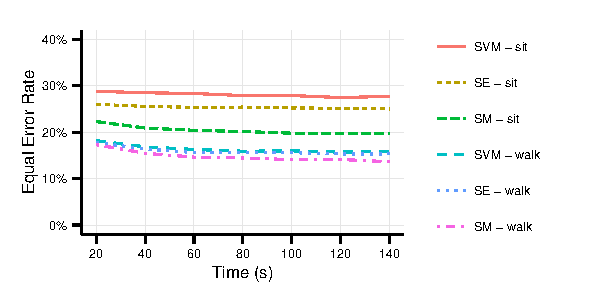
\includegraphics[width=1\linewidth]{plots_R/auth_hmog_all_verifiers_new.pdf}
\caption[]{Comparison of HMOG features in sitting and walking conditions for three verifiers. The reported EERs are with PCA for SE, and for SVM-sitting; and without PCA for SM and SVM-walking. $X$-axis shows authentication time in seconds.}
%
\label{fig:hmogAllVerifiersSitWalk}
\end{figure}

\begin{figure}[t]
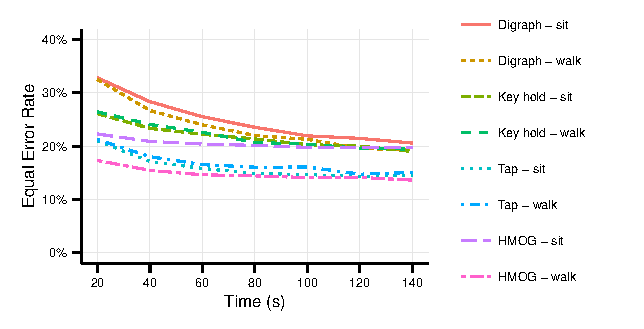
\includegraphics[width=1\linewidth]{plots_R/auth_compare_all_single.pdf}
\caption[]{Comparison of EERs of HMOG with keystroke dynamics (i.e., key hold and digraph) and tap features with SM verifier. $X$-axis shows authentication time in seconds.} %
\label{fig:walkVSsitAllSM}
\end{figure}

\paragraph{Comparison of HMOG with Keystroke Dynamics and Tap Features}
%
%
Tap features and HMOG features in walking condition performed better than keystroke dynamics features; HMOG in sitting outperforms keystroke dynamics for shorter scans and is comparable for longer scans (see Figure \ref{fig:walkVSsitAllSM}). 

HMOG features outperformed tap features in walking condition, while tap outperformed HMOG in sitting. 
The performance of tap and keystroke dynamics features did not change significantly between sitting and walking. However, the performance of HMOG improved considerably (up to 6.11\%) during walking. %

\begin{figure}[t]
 \centering
\subfigure[Sitting]
{
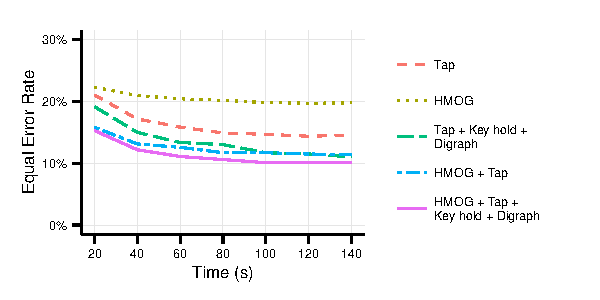
\includegraphics[width=1.1\linewidth]{plots_R/auth_fusion_sit.pdf}
\label{fig:sitFusionSM}}
\subfigure[Walking]
{
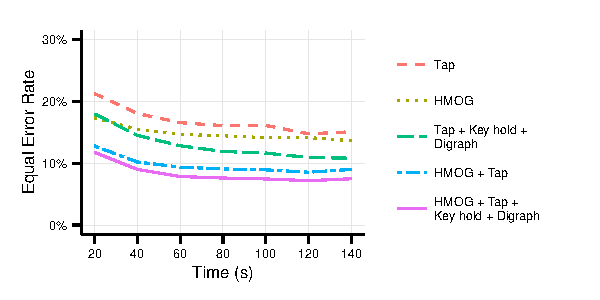
\includegraphics[width=1.1\linewidth]{plots_R/auth_fusion_walk.pdf}
\label{fig:walkFusionSM}}
\caption{Score-level fusion of combinations of feature types with SM verifier. $X$ axes show authentication time in seconds.}
\end{figure}





\paragraph{Fusion of HMOG, Tap, and Keystroke Features} We used SM verifier and performed score-level fusion with the following feature combinations: \{HMOG, tap, keystroke dynamics\};  \{tap, keystroke dynamics\}; and \{tap, HMOG\}. Detailed fusion results for sitting  and walking conditions are presented in figures \ref{fig:sitFusionSM} and~\ref{fig:walkFusionSM}, respectively. The lowest EERs achieved with fusion are summarized in Table~\ref{tab:fusionperformance},v and the corresponding DET curves for fusion on 60- and 120-second scan lengths are shown in Figure~\ref{fig:DETS}. %

%


%


%

%
 
%



%
%
Our results show that: (1) for both walking and sitting conditions, score-level fusion of all signals led to the lowest EER; and (2) fusing HMOG with tap features led to a decrease in EERs and either outperformed (in the case of walking and shorter scans in sitting) or was comparable (in the case of longer scans in sitting) to fusion of tap and keystroke dynamics (see figures~\ref{fig:sitFusionSM}) and \ref{fig:walkFusionSM}). Both (1) and (2) indicate that HMOG provides additional distinctiveness to that of tap and keystroke dynamics, especially in walking condition.



\begin{figure*}[t]
 \centering
\subfigure[Sitting (60-second scans)]
{
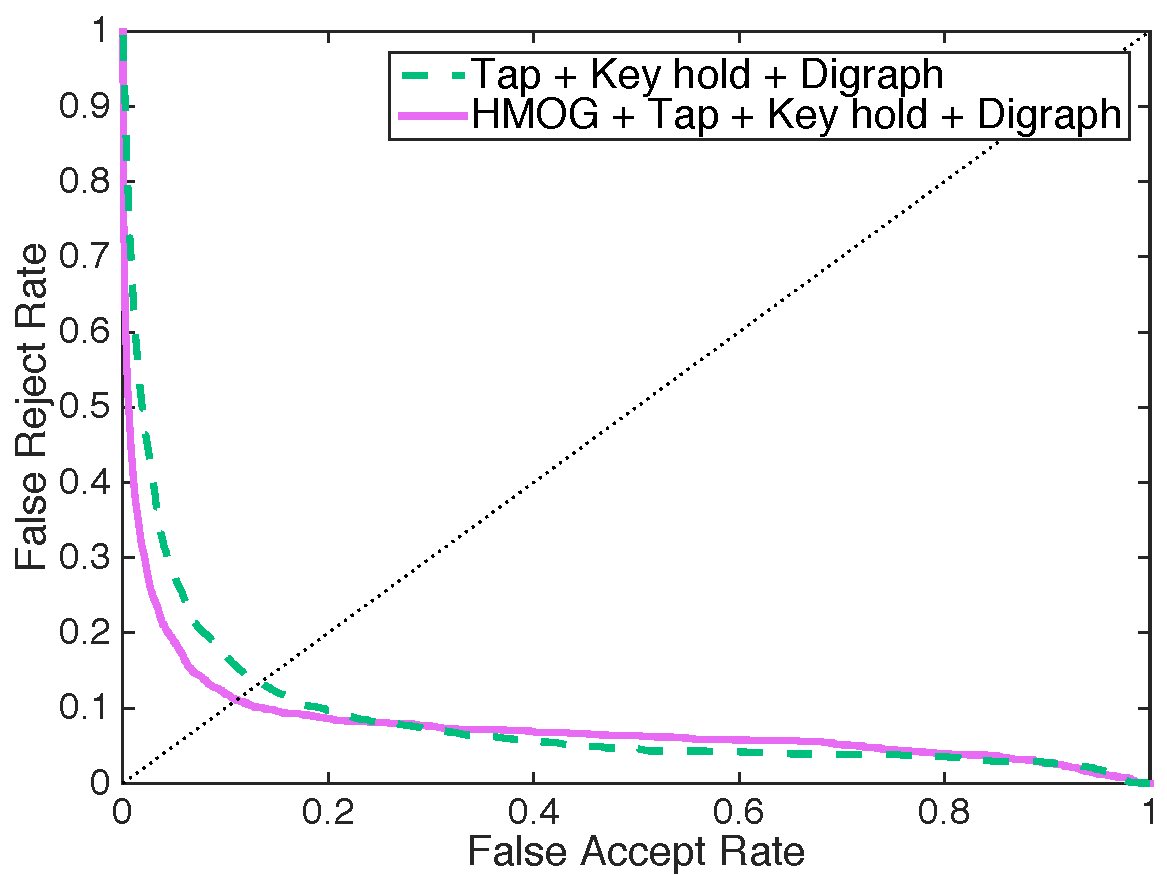
\includegraphics[width=0.4\linewidth]{plots/det_sit60.pdf}
\label{fig:DETsitFusionSM60}}
\subfigure[Walking (60-second scans)]
{
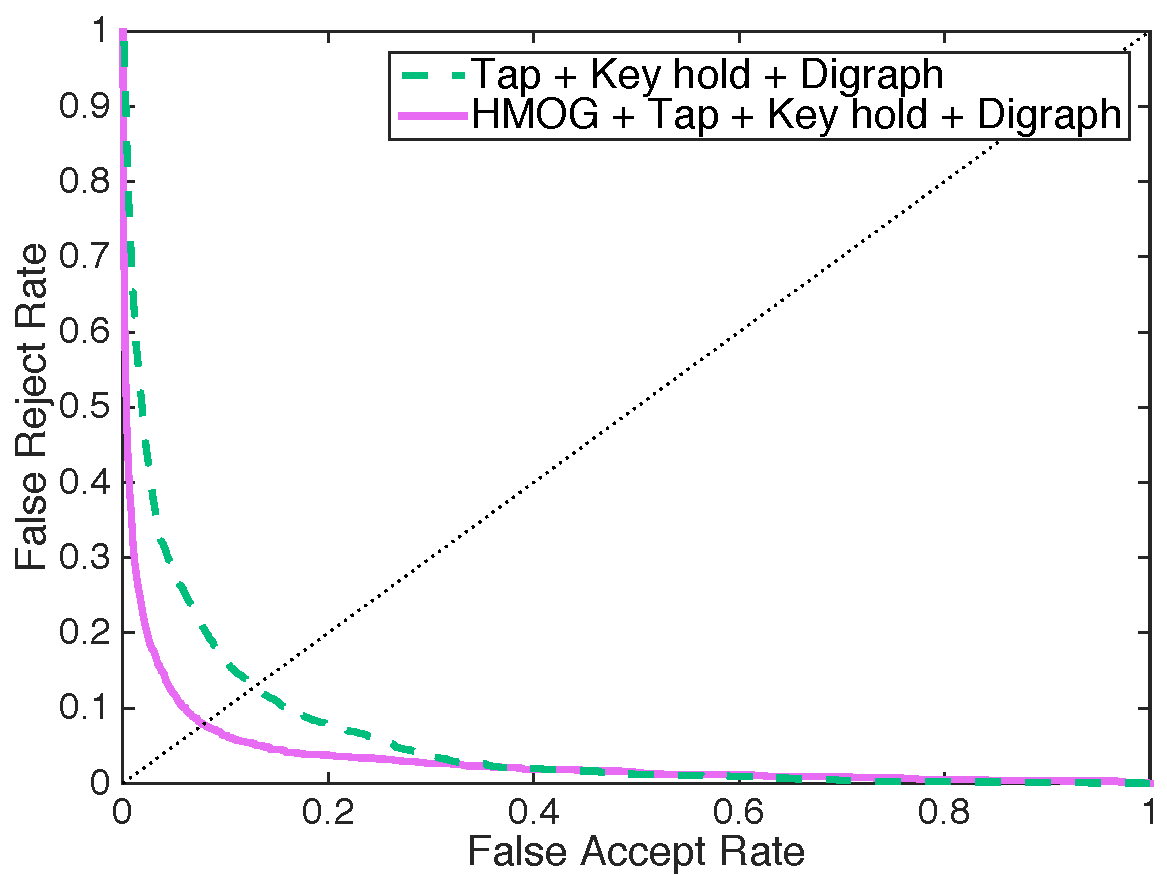
\includegraphics[width=0.4\linewidth]{plots/det_walk60.pdf}
\label{fig:DETwalkFusionSM60}}
\subfigure[Sitting (120-second scans)]
{
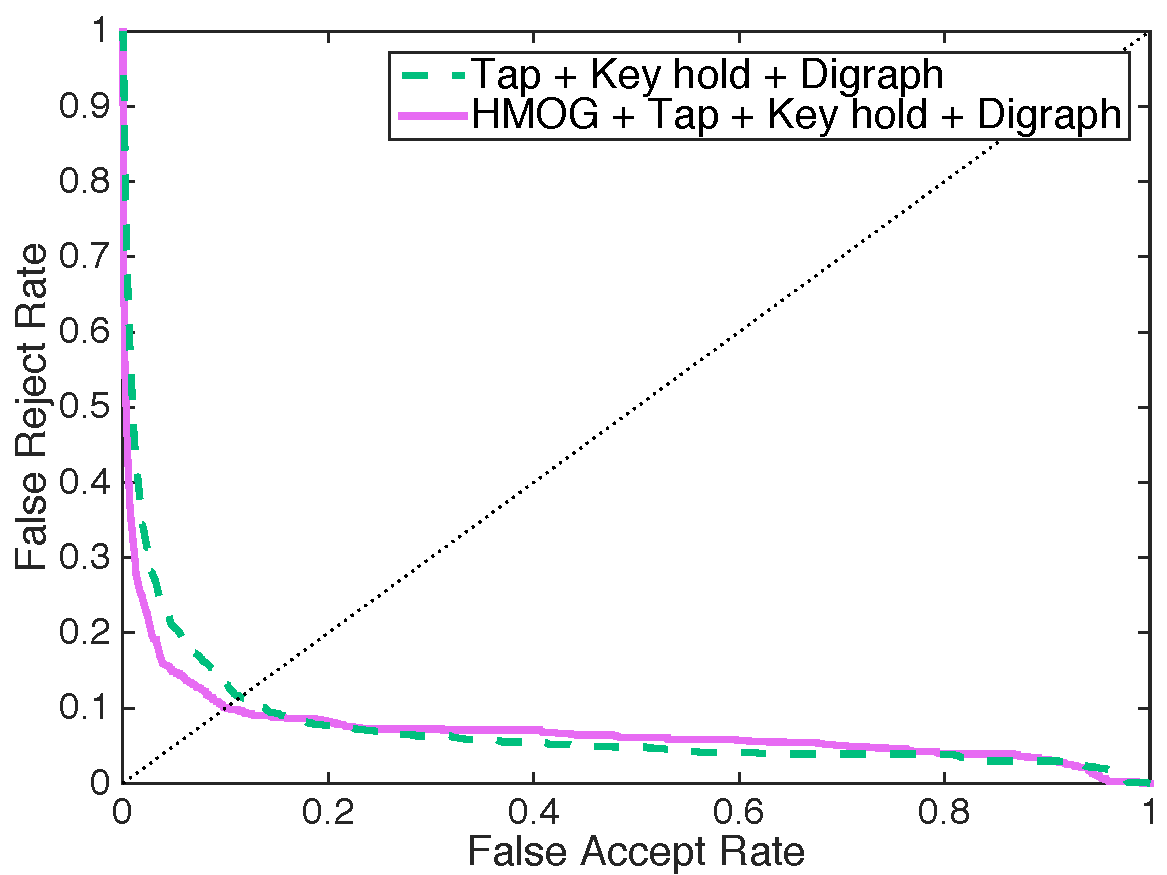
\includegraphics[width=0.4\linewidth]{plots/det_sit120.pdf}
\label{fig:DETsitFusionSM120}}
\subfigure[Walking (120-second scans)]
{
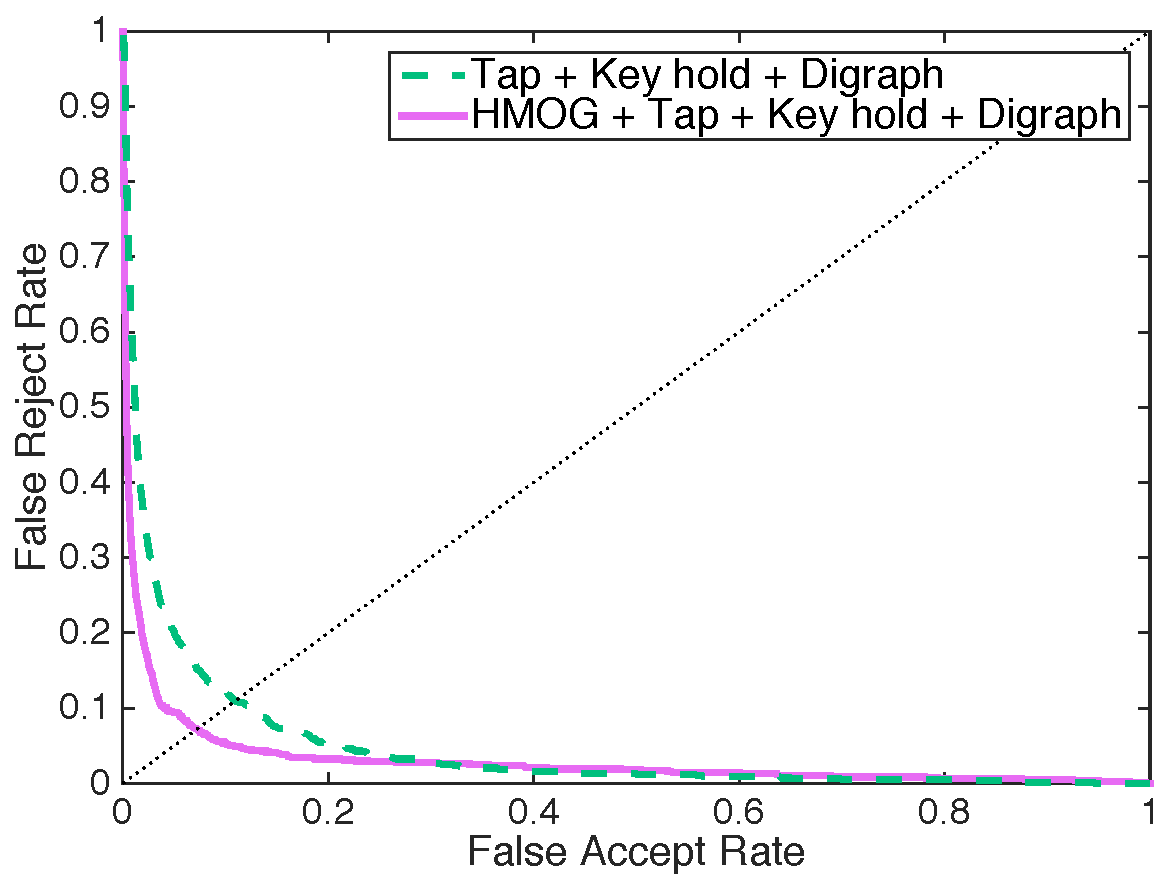
\includegraphics[width=0.4\linewidth]{plots/det_walk120.pdf}
\label{fig:DETwalkFusionSM120}}
\caption{DET curves for fusion of all feature types including and excluding HMOG. The scan lengths are 60- and 120-seconds.}
\label{fig:DETS}
\end{figure*}

%
%
%
%

%

%

 %

%

%

%

%

%
%
%
%
%
%
%
%
%
%
%
%




%

%
%
%
%
%


%
%

%


%

%

%

%

%

%

%

%

%
%

%
%


%



%
%
%
%
%
%
%
%
%
%
%
%
%
%
%
%
%
%
%




%
%

\begin{figure*}[t]
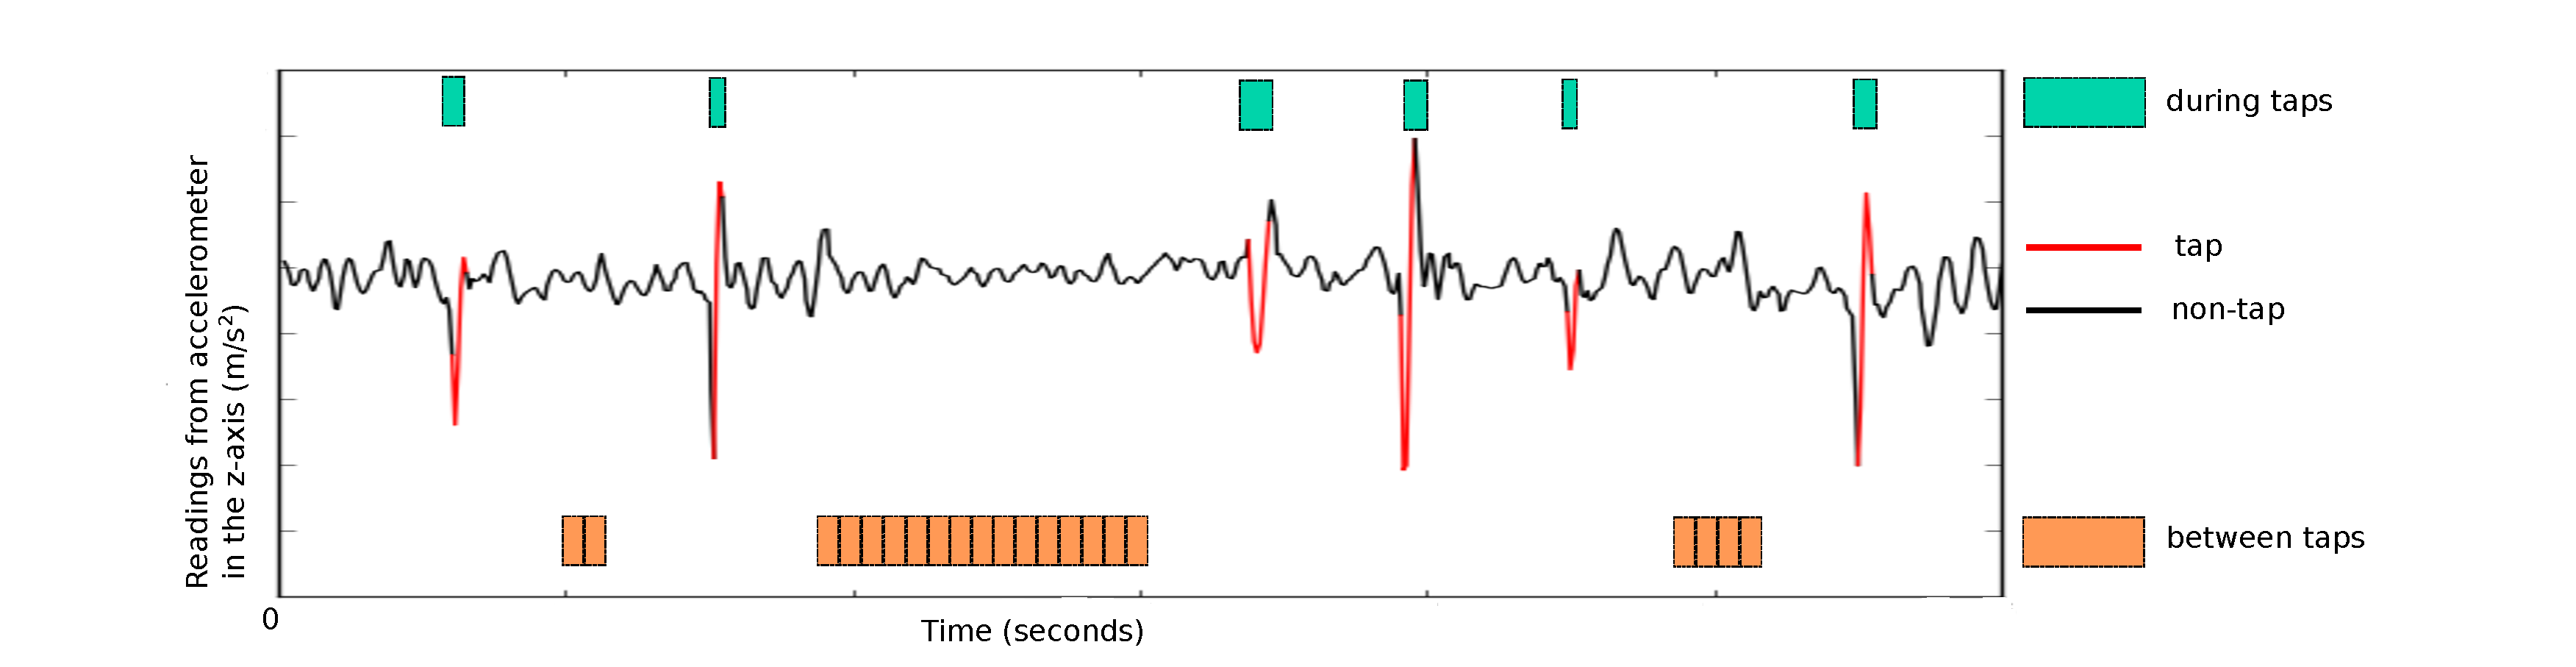
\includegraphics[width=1\linewidth]{plots/betweenExplainedFinal.pdf}
%
%
%
%
\caption[]{HMOG features extracted {\em during} and {\em between} taps. The figure shows a sample of readings from the z-axis of accelerometer in sitting condition.}
\label{fig:betweenExplained}
\end{figure*}








\subsection{Why HMOG Features Perform Better During Walking}

\begin{figure}[t]
%
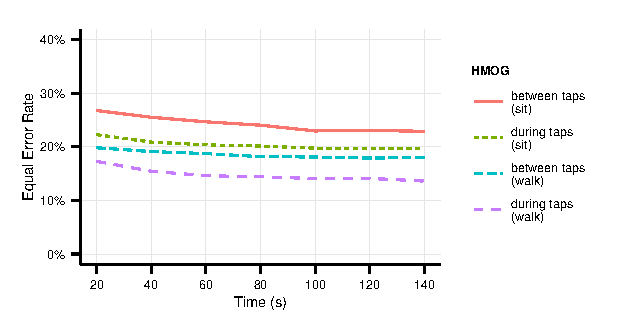
\includegraphics[width=1.1\linewidth]{plots_R/auth_between_taps.pdf}
\caption[]{Performance of HMOG features extracted {\em during}  and {\em between} taps. $X$-axis shows authentication time in seconds.}
\label{fig:betweenTapsSM}
%
%
%
%
%
%
\end{figure}

%

%

%

 %

%


%

We investigated why HMOG features performed better during walking. Specifically, we investigated whether the high authentication accuracies of HMOG features during walking were due to hand movements caused by taps, or due to movements caused by walking, or a combination of both. %

\paragraph{Experiment setup} We extracted 64 HMOG features from two segments of an accelerometer/gyroscope signal: (1) {\em during tap}, as discussed in previous sections; and (2) {\em between taps}, in which HMOG features were extracted when the user was \textit{not} tapping the screen (see Figure~\ref{fig:betweenExplained}). In (2), the signal between taps was segmented into non-overlapping blocks of 91~ms; one HMOG feature vector was extracted from each block. 
We selected 91ms as the block size because it was the median duration of a tap in our training data. This ensured that the number of sensor readings used to extract a HMOG feature vector {\em between} and {\em during} tap remained same. %

%

HMOG features extracted {\em during} taps use sensor readings from 100~ms before and 200~ms after a tap event (see Section \ref{sectionFeatures}). We extracted HMOG features {\em between} taps starting 300~ms after a tap until 300~ms before the next tap, to avoid any overlap between {\em during} and {\em between} HMOG features.%
%
%
%
%
%
 



%

%


%

%
%
%
%
%


%

%

%

%



%
%
The average number of the training vectors per user for HMOG {\em during} taps was 1122 for sitting, and 1186 for walking. For {\em between} taps, it was 7692 for sitting and 7462 for walking. %
The average number of testing vectors per user for HMOG features {\em during} taps was 897 for sitting and 972 for walking. For  {\em between} taps, it was 5885 for sitting and 5768 for walking. Verification experiments were performed using SM. 

%
%
%

%

\paragraph{Performance of HMOG Features Extracted During vs. Between Taps}  
We compared HMOG features extracted during taps with the same features extracted between taps for sitting and walking conditions. For sitting, HMOG features extracted {\em during} taps performed consistently better  than those extracted {\em between} taps (see EERs in Figure~\ref{fig:betweenTapsSM}). This indicates that HMOG features were able to capture distinctive hand micro-movement patterns when the users tapped on the phone. %
%
%
Similarly, for walking, HMOG features extracted {\em during} taps performed better than those extracted {\em between} taps (see EERs in Figure~\ref{fig:betweenTapsSM}). This again indicates that HMOG features capture user's distinctive hand micro-movement patterns when the user is tapping, regardless of the motion condition.
%


%
%

\paragraph{Impact of Walking on HMOG Features Extracted Between Taps} HMOG features extracted  {\em between} taps during walking outperformed the same when extracted during sitting (see {\em between} tap EERs for sitting and walking in Figure~\ref{fig:betweenTapsSM}). This indicates that HMOG features capture distinctive movements induced by walking, even in the {\em absence} of tap activity.%
%
%


\bigskip
Supported by the above results, the high authentication accuracies achieved by HMOG features during walking can be jointly attributed to: (a) the distinctiveness in hand movements caused by tap activity and (b) the distinctiveness in movements caused by walking. %


%

%
%

%

%
%
%

%

%
%

%

%


%

%


%
  
%


%


%

%

%



%





%

%

 %



%

%




%

%
%
%
%
%
%
%
%
%
%
%
%
%
%

%
%
%
%
%
%
%
%
%
%
%
%
%
%


%

%

%
%
%
%
%



%

%

%
%
%
%
%




%

%

%

%

%
 
%
%
%
%
%
%
%
%
%
%
%
%
%
%
%
%
%
%
%
%
%
%
%
%
%
%
%
%
%
%
%
%
%
%
%
%

%

%

%

%

%

%



%
%
%
%
%
%
%

%




%

%





 


%


%





%





%
%
%
%
%
%
%
%
%
%
%
%
%
%
%
%
%
%
%
%
%
%
%
%
%
%
%
%
%
%
%
%
%
%
%
%
